\subsection{Interfejs}

\begin{figure}[H]
\centering
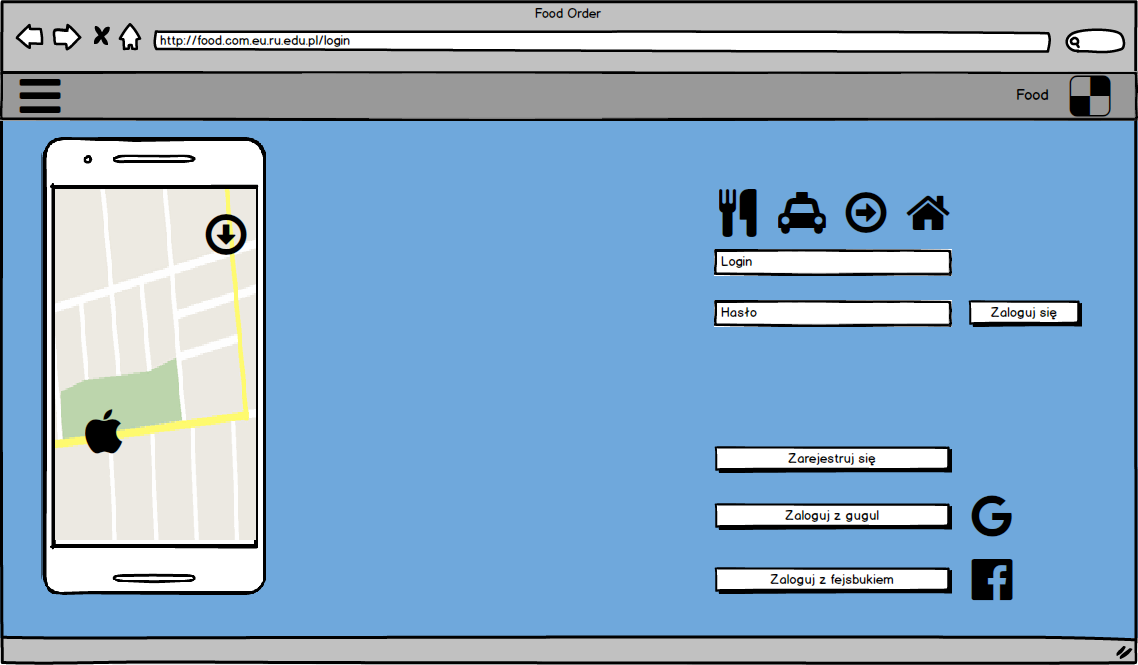
\includegraphics[width=15cm]{pictures/Logowanie_v2.png}
\caption{Efekt końcowy - ekran logowania.}
\end{figure}

\begin{figure}[H]
\centering
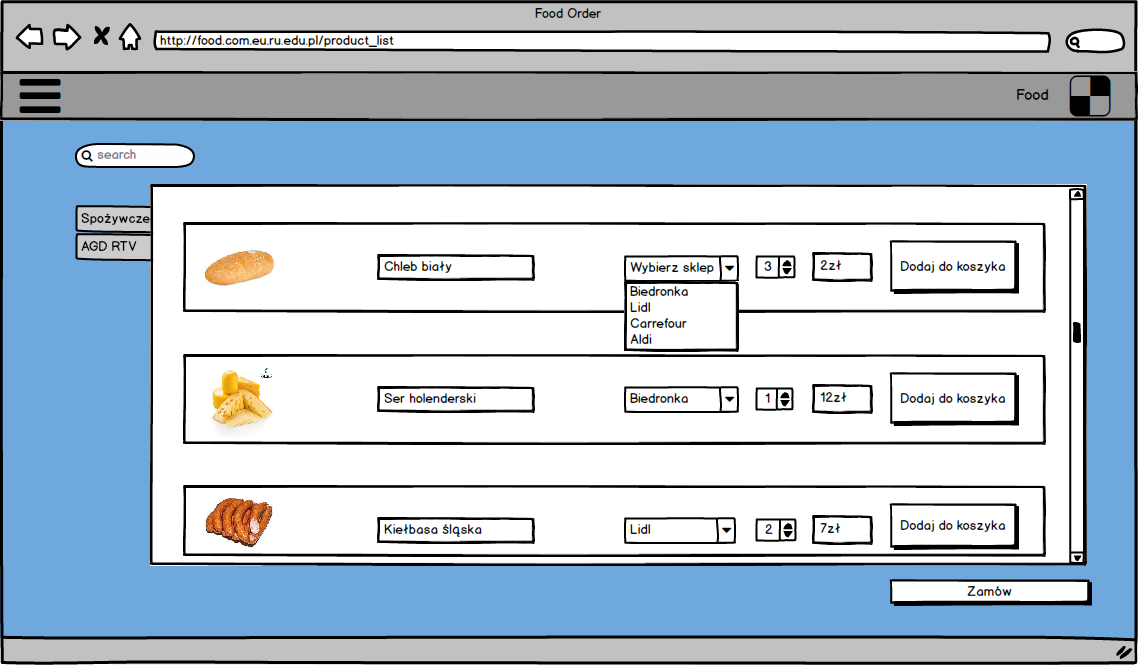
\includegraphics[width=15cm]{pictures/Lista_produktow_v3.png}
\caption{Efekt końcowy - lista produktów.}
\end{figure}

\begin{figure}[H]
\centering
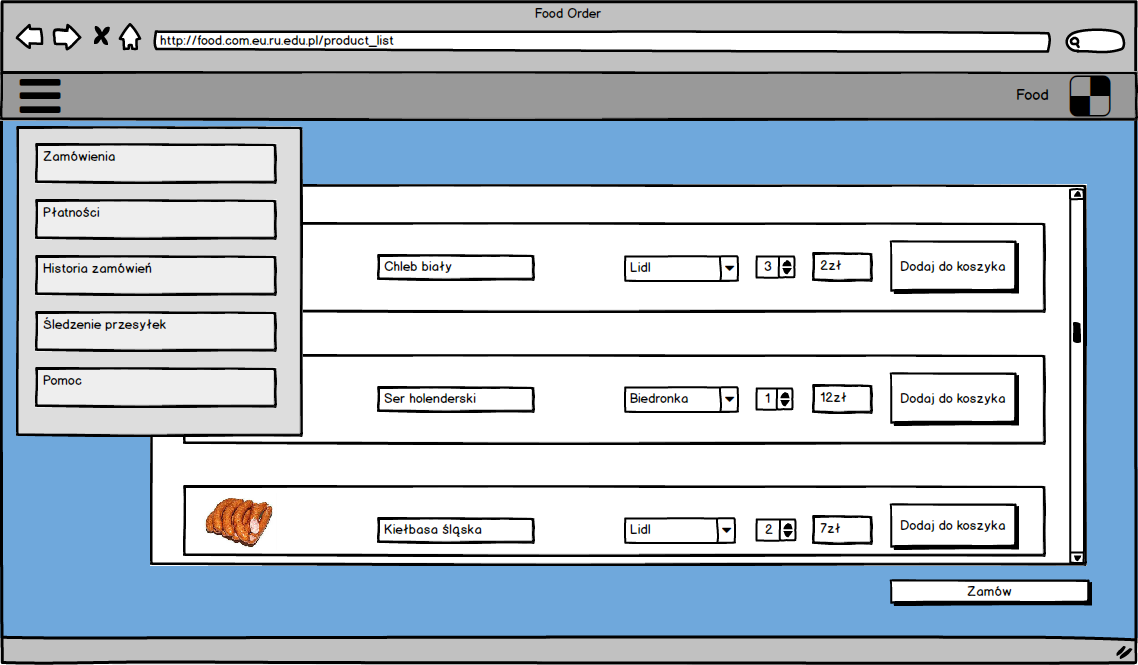
\includegraphics[width=15cm]{pictures/Navbar_v1.png}
\caption{Efekt końcowy - rozsunięte \textit{menu hamburger}.}
\end{figure}

\begin{figure}[H]
\centering
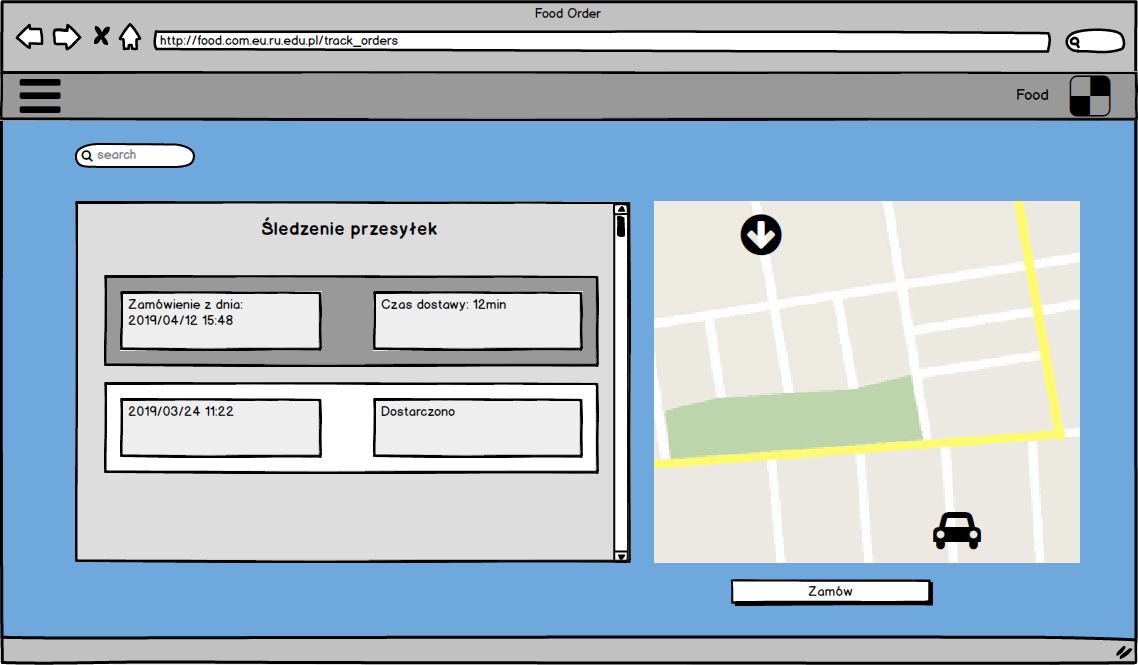
\includegraphics[width=15cm]{pictures/sledzenie_przesylek_v1.png}
\caption{Efekt końcowy - ekran śledzenia przesyłek.}
\end{figure}

\begin{figure}[H]
\centering
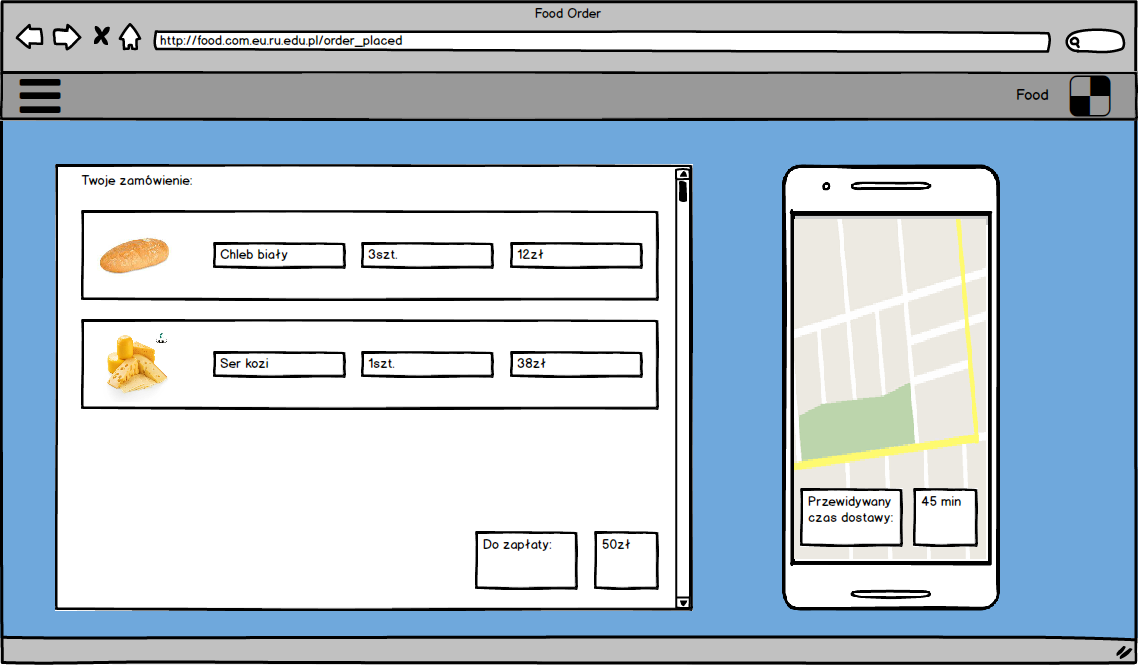
\includegraphics[width=15cm]{pictures/Zamowienie_zlozone_v3.png}
\caption{Efekt końcowy - ekran złożonego zamówienia.}
\end{figure}

\subsection{Ocena zamawiającego}
Poniżej cytat oceny interfejsu przez zamawiającego:
\begin{quote}
Aplikacja spełnia moje oczekiwania. Wyglada bardzo estetycznie i prosto tak jak zaplanowałem. W skali 5'cio punktowej skali oceniam ją na 4,5. 
\end{quote}